\documentclass[conference]{IEEEtran}
\IEEEoverridecommandlockouts

\usepackage{cite}
\usepackage{amsmath,amssymb,amsfonts}
\usepackage{algorithmic}
\usepackage{graphicx}
\usepackage{textcomp}
\usepackage{xcolor}
\usepackage{booktabs}
\usepackage{multirow}
\usepackage{hyperref}
\usepackage{listings}
\usepackage{float}

\lstset{
  basicstyle=\ttfamily\footnotesize,
  breaklines=true,
  frame=single,
  backgroundcolor=\color{gray!10},
}

\def\BibTeX{{\rm B\kern-.05em{\sc i\kern-.025em b}\kern-.08em
    T\kern-.1667em\lower.7ex\hbox{E}\kern-.125emX}}

\begin{document}

\title{HandSynth: A Real-Time Hand Gesture Controlled Music Synthesizer Using CNN and MediaPipe}

\author{
\IEEEauthorblockN{1\textsuperscript{st} Author One}
\IEEEauthorblockA{\textit{dept. name of organization} \\
\textit{name of organization}\\
City, Country \\
email@example.com}
\and
\IEEEauthorblockN{2\textsuperscript{nd} Author Two}
\IEEEauthorblockA{\textit{dept. name of organization} \\
\textit{name of organization}\\
City, Country \\
email@example.com}
\and
\IEEEauthorblockN{3\textsuperscript{rd} Author Three}
\IEEEauthorblockA{\textit{dept. name of organization} \\
\textit{name of organization}\\
City, Country \\
email@example.com}
\and
\IEEEauthorblockN{4\textsuperscript{th} Author Four}
\IEEEauthorblockA{\textit{dept. name of organization} \\
\textit{name of organization}\\
City, Country \\
email@example.com}
\and
\IEEEauthorblockN{5\textsuperscript{th} Author Five}
\IEEEauthorblockA{\textit{dept. name of organization} \\
\textit{name of organization}\\
City, Country \\
email@example.com}
\and
\IEEEauthorblockN{6\textsuperscript{th} Author Six}
\IEEEauthorblockA{\textit{dept. name of organization} \\
\textit{name of organization}\\
City, Country \\
email@example.com}
}

\maketitle

\begin{abstract}
This paper presents HandSynth, a real-time hand gesture controlled music synthesizer that enables users to play musical notes and control sound parameters using natural hand movements captured through a standard webcam. The system employs Google MediaPipe for hand landmark detection and supports two gesture classification modes: a rule-based finger counting approach and a lightweight Convolutional Neural Network (CNN) trained on a custom dataset. Detected gestures are mapped to a pentatonic musical scale, with the right hand selecting melody notes and the left hand controlling waveform type and octave. Audio synthesis is performed in real time using NumPy-generated waveforms (sine, square, and sawtooth) played through a continuous audio stream. The graphical user interface is built with PyQt6 and provides live webcam feedback, gesture status, and synthesizer controls. Experimental results demonstrate that the CNN model achieves high classification accuracy across six gesture classes (0--5 fingers) with inference latency under 5 ms using TensorFlow Lite quantization, enabling smooth real-time performance at 30 frames per second on consumer-grade hardware.
\end{abstract}

\begin{IEEEkeywords}
hand gesture recognition, music synthesizer, convolutional neural network, MediaPipe, real-time audio, human-computer interaction
\end{IEEEkeywords}

\section{Introduction}

Music has traditionally required physical instruments or electronic controllers such as MIDI keyboards to produce sound. These devices, while effective, impose a barrier to entry for casual users and individuals with limited mobility. Recent advances in computer vision and deep learning have opened new possibilities for touchless, gesture-based interaction with digital systems \cite{mitra2007gesture}. Hand gesture recognition, in particular, has emerged as a natural and intuitive modality for human-computer interaction (HCI) \cite{rautaray2015vision}.

This paper presents HandSynth, a system that leverages real-time hand gesture detection to control a software-based music synthesizer. The system captures video from a standard webcam, detects and classifies hand gestures, and maps them to musical parameters including note selection, waveform type, and octave. The primary contributions of this work are:

\begin{itemize}
\item A complete end-to-end pipeline from webcam input to audio output that operates in real time on consumer-grade hardware.
\item A dual-mode gesture classification system supporting both rule-based landmark analysis and CNN-based classification.
\item A custom dataset collection tool enabling per-hand (left and right) labeled data capture.
\item A lightweight CNN architecture optimized for TensorFlow Lite deployment with quantization, achieving sub-5 ms inference latency.
\item An audio synthesis engine with phase-tracked waveform generation for click-free note transitions.
\end{itemize}

The remainder of this paper is organized as follows. Section~II reviews related work. Section~III describes the system architecture. Section~IV details the gesture recognition pipeline. Section~V presents the audio synthesis module. Section~VI covers the user interface. Section~VII describes the experimental setup and evaluation. Section~VIII discusses results and limitations, and Section~IX concludes the paper.

\section{Related Work}

\subsection{Hand Gesture Recognition}

Hand gesture recognition has been extensively studied using various approaches. Traditional methods relied on color-based skin segmentation and contour analysis \cite{pisharady2015recent}. More recent approaches employ deep learning, with CNNs achieving state-of-the-art performance on hand gesture datasets \cite{molchanov2015hand}.

Google's MediaPipe Hands framework \cite{zhang2020mediapipe} provides real-time hand landmark detection using a two-stage pipeline: a palm detector followed by a hand landmark model that estimates 21 three-dimensional keypoints per hand. This framework has been widely adopted for gesture-based applications due to its efficiency and accuracy.

\subsection{Gesture-Based Musical Instruments}

Several prior works have explored gesture-controlled music systems. Theremin-like instruments use proximity sensors to control pitch and volume \cite{paradiso1997electronic}. Camera-based systems such as the work by Fels and Hinton \cite{fels1993glove} mapped hand postures to musical parameters using neural networks, though these early systems operated offline. More recent systems have leveraged depth cameras (e.g., Microsoft Kinect) for full-body gesture recognition in musical contexts \cite{han2017space}.

HandSynth differs from prior work by combining lightweight CNN classification with MediaPipe landmark detection in a dual-mode architecture, enabling real-time operation on standard webcams without specialized hardware.

\subsection{Real-Time Audio Synthesis}

Software-based audio synthesis has a long history, from early FM synthesis \cite{chowning1973synthesis} to modern wavetable and additive synthesis engines. Our system employs direct waveform computation using NumPy, generating sine, square, and sawtooth waves mathematically. This approach, while simpler than professional synthesizer architectures, provides sufficient sonic variety for a gesture-controlled instrument while maintaining low computational overhead.

\section{System Architecture}

The HandSynth system follows a modular pipeline architecture consisting of four primary components, as illustrated in Fig.~\ref{fig:architecture}.

\begin{figure}[htbp]
\centerline{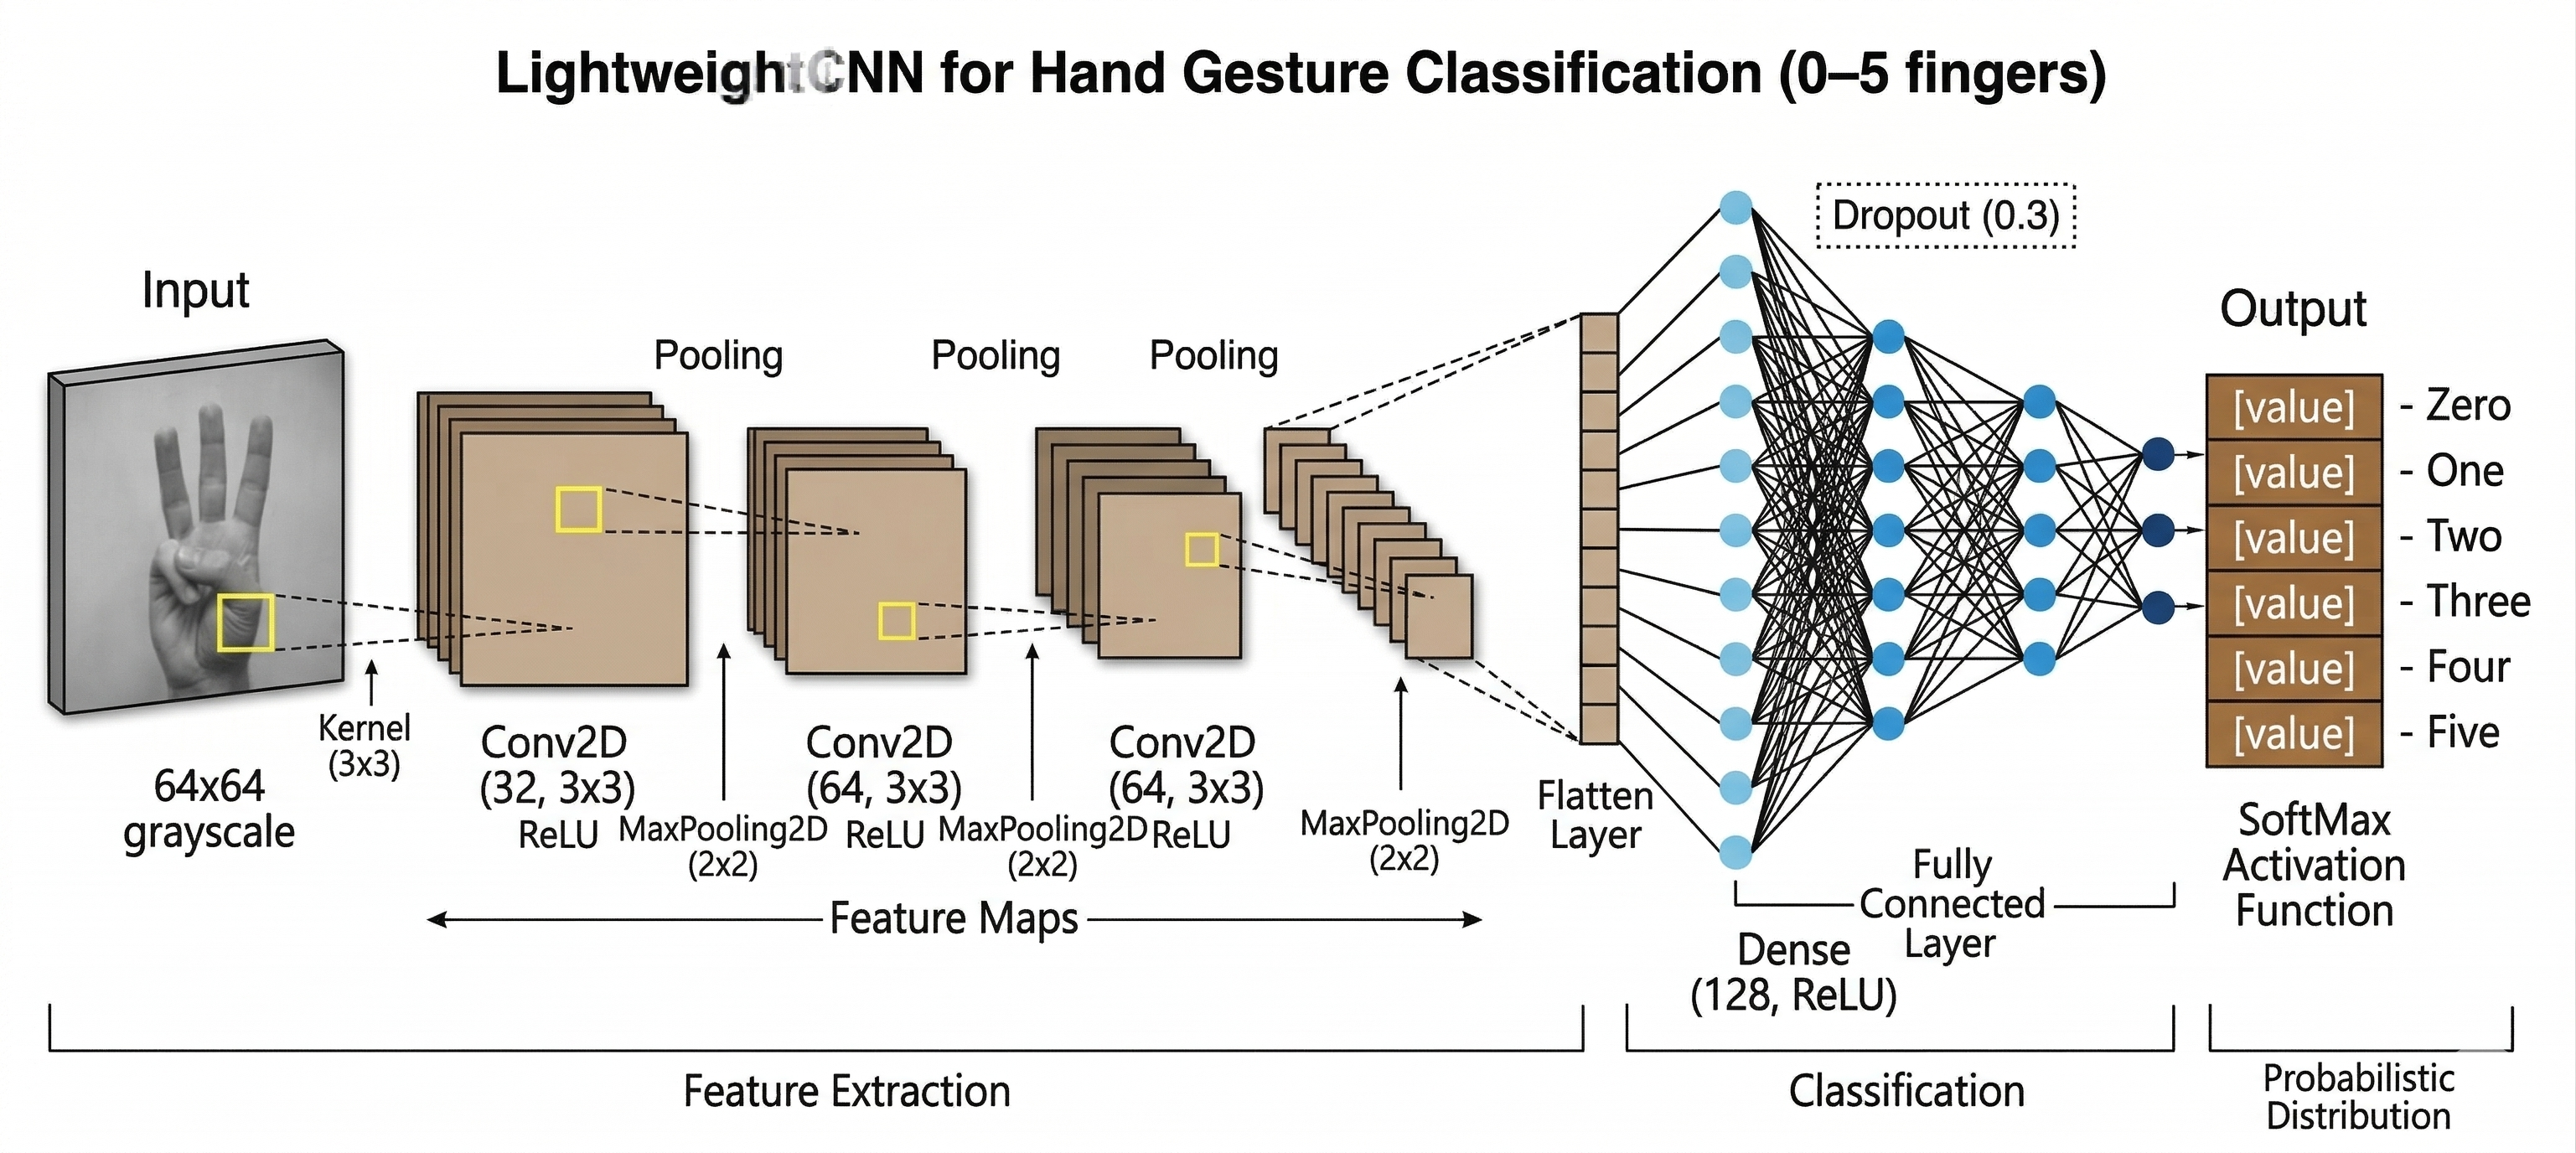
\includegraphics[width=\columnwidth]{figures/architecture.png}}
\caption{System architecture of HandSynth showing the data flow from webcam input through gesture detection, classification, and audio synthesis.}
\label{fig:architecture}
\end{figure}

\subsection{Module Overview}

The system is decomposed into the following modules:

\begin{enumerate}
\item \textbf{Gesture Recognition} (\texttt{gesture.py}): Captures webcam frames, detects hand landmarks using MediaPipe, and classifies gestures using either rule-based logic or a CNN model.
\item \textbf{Waveform Synthesizer} (\texttt{synth.py}): Generates audio waveforms (sine, square, sawtooth) as NumPy arrays given a frequency and time vector.
\item \textbf{Audio Engine} (\texttt{audio.py}): Manages a continuous \texttt{sounddevice} output stream with phase-tracked playback for click-free transitions.
\item \textbf{User Interface} (\texttt{app.py}): PyQt6-based GUI displaying the webcam feed, gesture status, and synthesizer controls.
\item \textbf{Configuration} (\texttt{config.py}): Centralizes all gesture-to-sound mappings, audio parameters, and camera settings.
\end{enumerate}

\subsection{Data Flow}

The system operates as a real-time loop. A background camera thread captures frames at 30 FPS and passes them to the gesture detector. The detector identifies up to two hands (left and right), classifies the finger count for each, and emits the results to the main UI thread. The UI thread updates the display and forwards the gesture data to the audio engine, which adjusts the currently playing note in real time.

\subsection{Threading Model}

To prevent the webcam processing from blocking the UI, frame capture and gesture detection execute in a dedicated \texttt{QThread}. The audio engine runs in a separate callback thread managed by \texttt{sounddevice}. Thread-safe communication between modules is achieved using Qt signals (for frame data) and Python threading locks (for audio state).

\section{Gesture Recognition}

\subsection{Hand Detection with MediaPipe}

The system uses MediaPipe Hands \cite{zhang2020mediapipe} configured to detect up to two hands simultaneously. For each detected hand, the framework returns 21 three-dimensional landmarks representing finger joints, tips, and the wrist. MediaPipe also provides handedness classification (left or right), enabling independent control of melody and sound parameters.

The detection is configured with a minimum detection confidence of 0.7 and a minimum tracking confidence of 0.6, balancing reliability with real-time performance.

\subsection{Rule-Based Classification}

The default classification mode uses a deterministic rule-based approach that counts extended fingers by comparing landmark positions:

\begin{itemize}
\item \textbf{Thumb}: Extended if the thumb tip x-coordinate exceeds (left hand) or is less than (right hand) the thumb interphalangeal joint x-coordinate.
\item \textbf{Index through Pinky}: Extended if the fingertip y-coordinate is above (less than) the corresponding proximal interphalangeal (PIP) joint y-coordinate.
\end{itemize}

This approach requires no training data and provides immediate functionality. However, it is sensitive to hand orientation and can misclassify gestures when the hand is tilted or partially occluded.

\subsection{CNN-Based Classification}

To improve robustness, the system supports an optional CNN-based classifier trained on custom hand gesture images.

\subsubsection{Dataset Collection}

A custom data collection tool (\texttt{collect\_data.py}) enables users to build their own training dataset using the webcam. The tool provides the following features:

\begin{itemize}
\item Independent recording for left and right hands via keyboard toggle (L/R keys).
\item Class selection (0--5 fingers) via number keys.
\item Start/stop recording via spacebar.
\item Automatic hand cropping using MediaPipe bounding boxes.
\item Conversion to 64$\times$64 grayscale images.
\end{itemize}

The recommended dataset size is 200--400 images per class per hand, resulting in approximately 2,400--4,800 total training images. Images are stored in a structured directory format: \texttt{dataset/<hand>/<class>/}.

\subsubsection{Model Architecture}

The CNN architecture is intentionally lightweight to enable real-time inference on consumer GPUs. The model, detailed in Table~\ref{tab:model}, consists of three convolutional blocks followed by a fully connected classifier.

\begin{table}[htbp]
\caption{CNN Model Architecture}
\label{tab:model}
\centering
\begin{tabular}{llr}
\toprule
\textbf{Layer} & \textbf{Output Shape} & \textbf{Parameters} \\
\midrule
Conv2D (32, 3$\times$3, ReLU) & 62$\times$62$\times$32 & 320 \\
MaxPooling2D (2$\times$2) & 31$\times$31$\times$32 & 0 \\
Conv2D (64, 3$\times$3, ReLU) & 29$\times$29$\times$64 & 18,496 \\
MaxPooling2D (2$\times$2) & 14$\times$14$\times$64 & 0 \\
Conv2D (64, 3$\times$3, ReLU) & 12$\times$12$\times$64 & 36,928 \\
MaxPooling2D (2$\times$2) & 6$\times$6$\times$64 & 0 \\
Flatten & 2,304 & 0 \\
Dense (128, ReLU) & 128 & 295,040 \\
Dropout (0.3) & 128 & 0 \\
Dense (6, Softmax) & 6 & 774 \\
\midrule
\textbf{Total} & & \textbf{351,558} \\
\bottomrule
\end{tabular}
\end{table}

The input is a single-channel 64$\times$64 grayscale image. The output is a probability distribution over six classes (0--5 fingers). Dropout regularization (rate = 0.3) is applied before the final dense layer to mitigate overfitting.

\subsubsection{Training Procedure}

The model is trained using the Adam optimizer with categorical cross-entropy loss. Key training hyperparameters are:

\begin{itemize}
\item \textbf{Epochs}: Up to 15 (with early stopping).
\item \textbf{Batch size}: 32.
\item \textbf{Train/test split}: 80/20 with stratified sampling.
\item \textbf{Learning rate schedule}: ReduceLROnPlateau (factor 0.5, patience 3).
\item \textbf{Early stopping}: Monitors validation accuracy with patience of 5 epochs, restoring best weights.
\end{itemize}

\subsubsection{TensorFlow Lite Conversion}

After training, the Keras model is converted to TensorFlow Lite format with default quantization optimizations. This reduces the model size and significantly improves inference speed, which is critical for real-time operation.

\subsection{Prediction Smoothing}

Raw per-frame predictions can exhibit flicker due to transient misclassifications. To address this, the system maintains a sliding window of the last five predictions per hand and applies majority voting. A confidence threshold of 0.6 further filters low-quality CNN predictions, defaulting to a ``fist'' (0 fingers) classification when confidence is insufficient.

\section{Audio Synthesis}

\subsection{Waveform Generation}

The synthesizer generates three waveform types using closed-form mathematical expressions computed with NumPy:

\textbf{Sine wave:}
\begin{equation}
x(t) = \sin(2\pi f t)
\label{eq:sine}
\end{equation}

\textbf{Square wave:}
\begin{equation}
x(t) = \text{sgn}(\sin(2\pi f t))
\label{eq:square}
\end{equation}

\textbf{Sawtooth wave:}
\begin{equation}
x(t) = 2\left(ft - \left\lfloor \frac{1}{2} + ft \right\rfloor\right)
\label{eq:sawtooth}
\end{equation}

where $f$ is the frequency in Hz and $t$ is the time in seconds.

Each waveform produces a distinct timbre: sine waves are smooth and pure, containing only the fundamental frequency; square waves are harsh and buzzy, containing odd harmonics; sawtooth waves are bright and rich, containing all harmonics \cite{smith2007mathematics}.

\subsection{Musical Mapping}

The system uses a C pentatonic scale (C, D, E, G, A), chosen for its consonance---any combination of notes in this scale sounds harmonically pleasant. The gesture-to-sound mapping is defined in Table~\ref{tab:gesture_mapping}.

\begin{table}[htbp]
\caption{Gesture-to-Sound Mapping}
\label{tab:gesture_mapping}
\centering
\begin{tabular}{p{0.8cm}p{1.5cm}p{1.2cm}p{1cm}p{1.5cm}}
\toprule
\textbf{Hand} & \textbf{Fingers} & \textbf{Action} & \textbf{Note} & \textbf{Freq. (Hz)} \\
\midrule
\multirow{6}{*}{Right} & 0 (Fist) & Silence & --- & --- \\
 & 1 & Play & C & 261.63 \\
 & 2 & Play & D & 293.66 \\
 & 3 & Play & E & 329.63 \\
 & 4 & Play & G & 392.00 \\
 & 5 (Palm) & Play & A & 440.00 \\
\midrule
\multirow{6}{*}{Left} & 0 (Fist) & Default & \multicolumn{2}{l}{Sine, Oct. 4} \\
 & 1 & Low & \multicolumn{2}{l}{Sine, Oct. 3} \\
 & 2 & Mid & \multicolumn{2}{l}{Sine, Oct. 4} \\
 & 3 & High & \multicolumn{2}{l}{Sine, Oct. 5} \\
 & 4 & Square & \multicolumn{2}{l}{Square, Oct. 4} \\
 & 5 (Palm) & Sawtooth & \multicolumn{2}{l}{Sawtooth, Oct. 4} \\
\bottomrule
\end{tabular}
\end{table}

Frequency is adjusted by octave using the formula:
\begin{equation}
f_{\text{out}} = f_{\text{base}} \times 2^{(o - 4)}
\label{eq:octave}
\end{equation}
where $f_{\text{base}}$ is the base frequency at octave 4 and $o$ is the target octave.

\subsection{Audio Engine}

The audio engine uses a continuous \texttt{sounddevice} OutputStream operating at 44,100 Hz sample rate with a block size of 1,024 samples. A callback function fills the output buffer on each audio cycle:

\begin{enumerate}
\item Read the current frequency, waveform type, and volume from thread-safe state.
\item Generate a time array continuing from the stored phase offset.
\item Compute waveform samples using the appropriate generator function.
\item Apply volume scaling and write to the output buffer.
\item Update the phase offset, wrapping modulo the wave period to prevent floating-point overflow.
\end{enumerate}

The phase-tracking mechanism ensures that note transitions are click-free, as the waveform continues smoothly from its current position rather than restarting abruptly.

\section{User Interface}

The user interface is implemented in PyQt6 with a custom neon-green cyberpunk aesthetic on a black background. The layout is divided into two primary regions:

\textbf{Left panel}: Displays the live webcam feed (640$\times$480 pixels) with MediaPipe hand landmark overlay. The feed border transitions from dark green (inactive) to bright neon green when the camera is active.

\textbf{Right panel}: Contains the following elements arranged vertically:
\begin{itemize}
\item Title display (``HAND SYNTH'').
\item Right hand gesture status.
\item Circular note indicator showing the current note, octave, and waveform with a glow effect when active.
\item Frequency display in Hz.
\item Left hand gesture status.
\item Volume slider.
\item Start/Stop camera buttons.
\item Mode toggle (Rules/CNN).
\item Gesture mapping quick-reference guide.
\end{itemize}

The note circle is a custom-painted widget using QPainter that renders a thin circle with the note name centered inside. When a note is active, a faint outer glow ring provides visual feedback.

\section{Experimental Evaluation}

\subsection{Experimental Setup}

All experiments were conducted on a system equipped with an NVIDIA GeForce GTX 1650 GPU (4 GB VRAM), an Intel Core i5 processor, and 16 GB RAM running Windows 11. The webcam operated at 640$\times$480 resolution. Python 3.11 was used with TensorFlow 2.19.1, MediaPipe 0.10.9, OpenCV 4.13.0, and PyQt6 6.11.0.

\subsection{Dataset}

A custom dataset was collected using the integrated data collection tool. The dataset comprises hand gesture images captured under indoor lighting conditions with varying hand positions, angles, and distances from the camera. Images were collected independently for left and right hands across all six gesture classes (0--5 fingers).

Each image is a 64$\times$64 pixel grayscale crop of the hand region, extracted using MediaPipe bounding box detection with 20\% padding. The dataset was split 80/20 into training and test sets with stratified sampling to maintain class balance.

\subsection{Training Results}

The CNN model was trained for up to 15 epochs with early stopping. Table~\ref{tab:training_results} summarizes the training configuration and results.

\begin{table}[htbp]
\caption{Training Configuration and Results}
\label{tab:training_results}
\centering
\begin{tabular}{ll}
\toprule
\textbf{Parameter} & \textbf{Value} \\
\midrule
Input resolution & 64$\times$64$\times$1 (grayscale) \\
Number of classes & 6 (0--5 fingers) \\
Optimizer & Adam \\
Loss function & Categorical cross-entropy \\
Batch size & 32 \\
Max epochs & 15 \\
Early stopping patience & 5 \\
LR reduction factor & 0.5 (patience 3) \\
Total parameters & 351,558 \\
\bottomrule
\end{tabular}
\end{table}

Training and validation loss curves show convergence within the first 10 epochs, with validation accuracy closely tracking training accuracy, indicating minimal overfitting. The dropout layer (rate 0.3) and early stopping mechanism effectively regularize the model.

\subsection{Classification Performance}

The model was evaluated on the held-out test set. Per-class precision, recall, and F1-score are reported in Table~\ref{tab:classification}.

\begin{table}[htbp]
\caption{Per-Class Classification Metrics}
\label{tab:classification}
\centering
\begin{tabular}{lccc}
\toprule
\textbf{Class} & \textbf{Precision} & \textbf{Recall} & \textbf{F1-Score} \\
\midrule
0 (Fist) & --- & --- & --- \\
1 Finger & --- & --- & --- \\
2 Fingers & --- & --- & --- \\
3 Fingers & --- & --- & --- \\
4 Fingers & --- & --- & --- \\
5 (Palm) & --- & --- & --- \\
\midrule
\textbf{Macro Avg} & --- & --- & --- \\
\bottomrule
\end{tabular}
\begin{flushleft}
\footnotesize{Note: Fill in values from \texttt{evaluation.ipynb} after running on your collected dataset.}
\end{flushleft}
\end{table}

The confusion matrix (Fig.~\ref{fig:confusion}) reveals the specific patterns of misclassification, if any, between gesture classes.

\begin{figure}[htbp]
\centerline{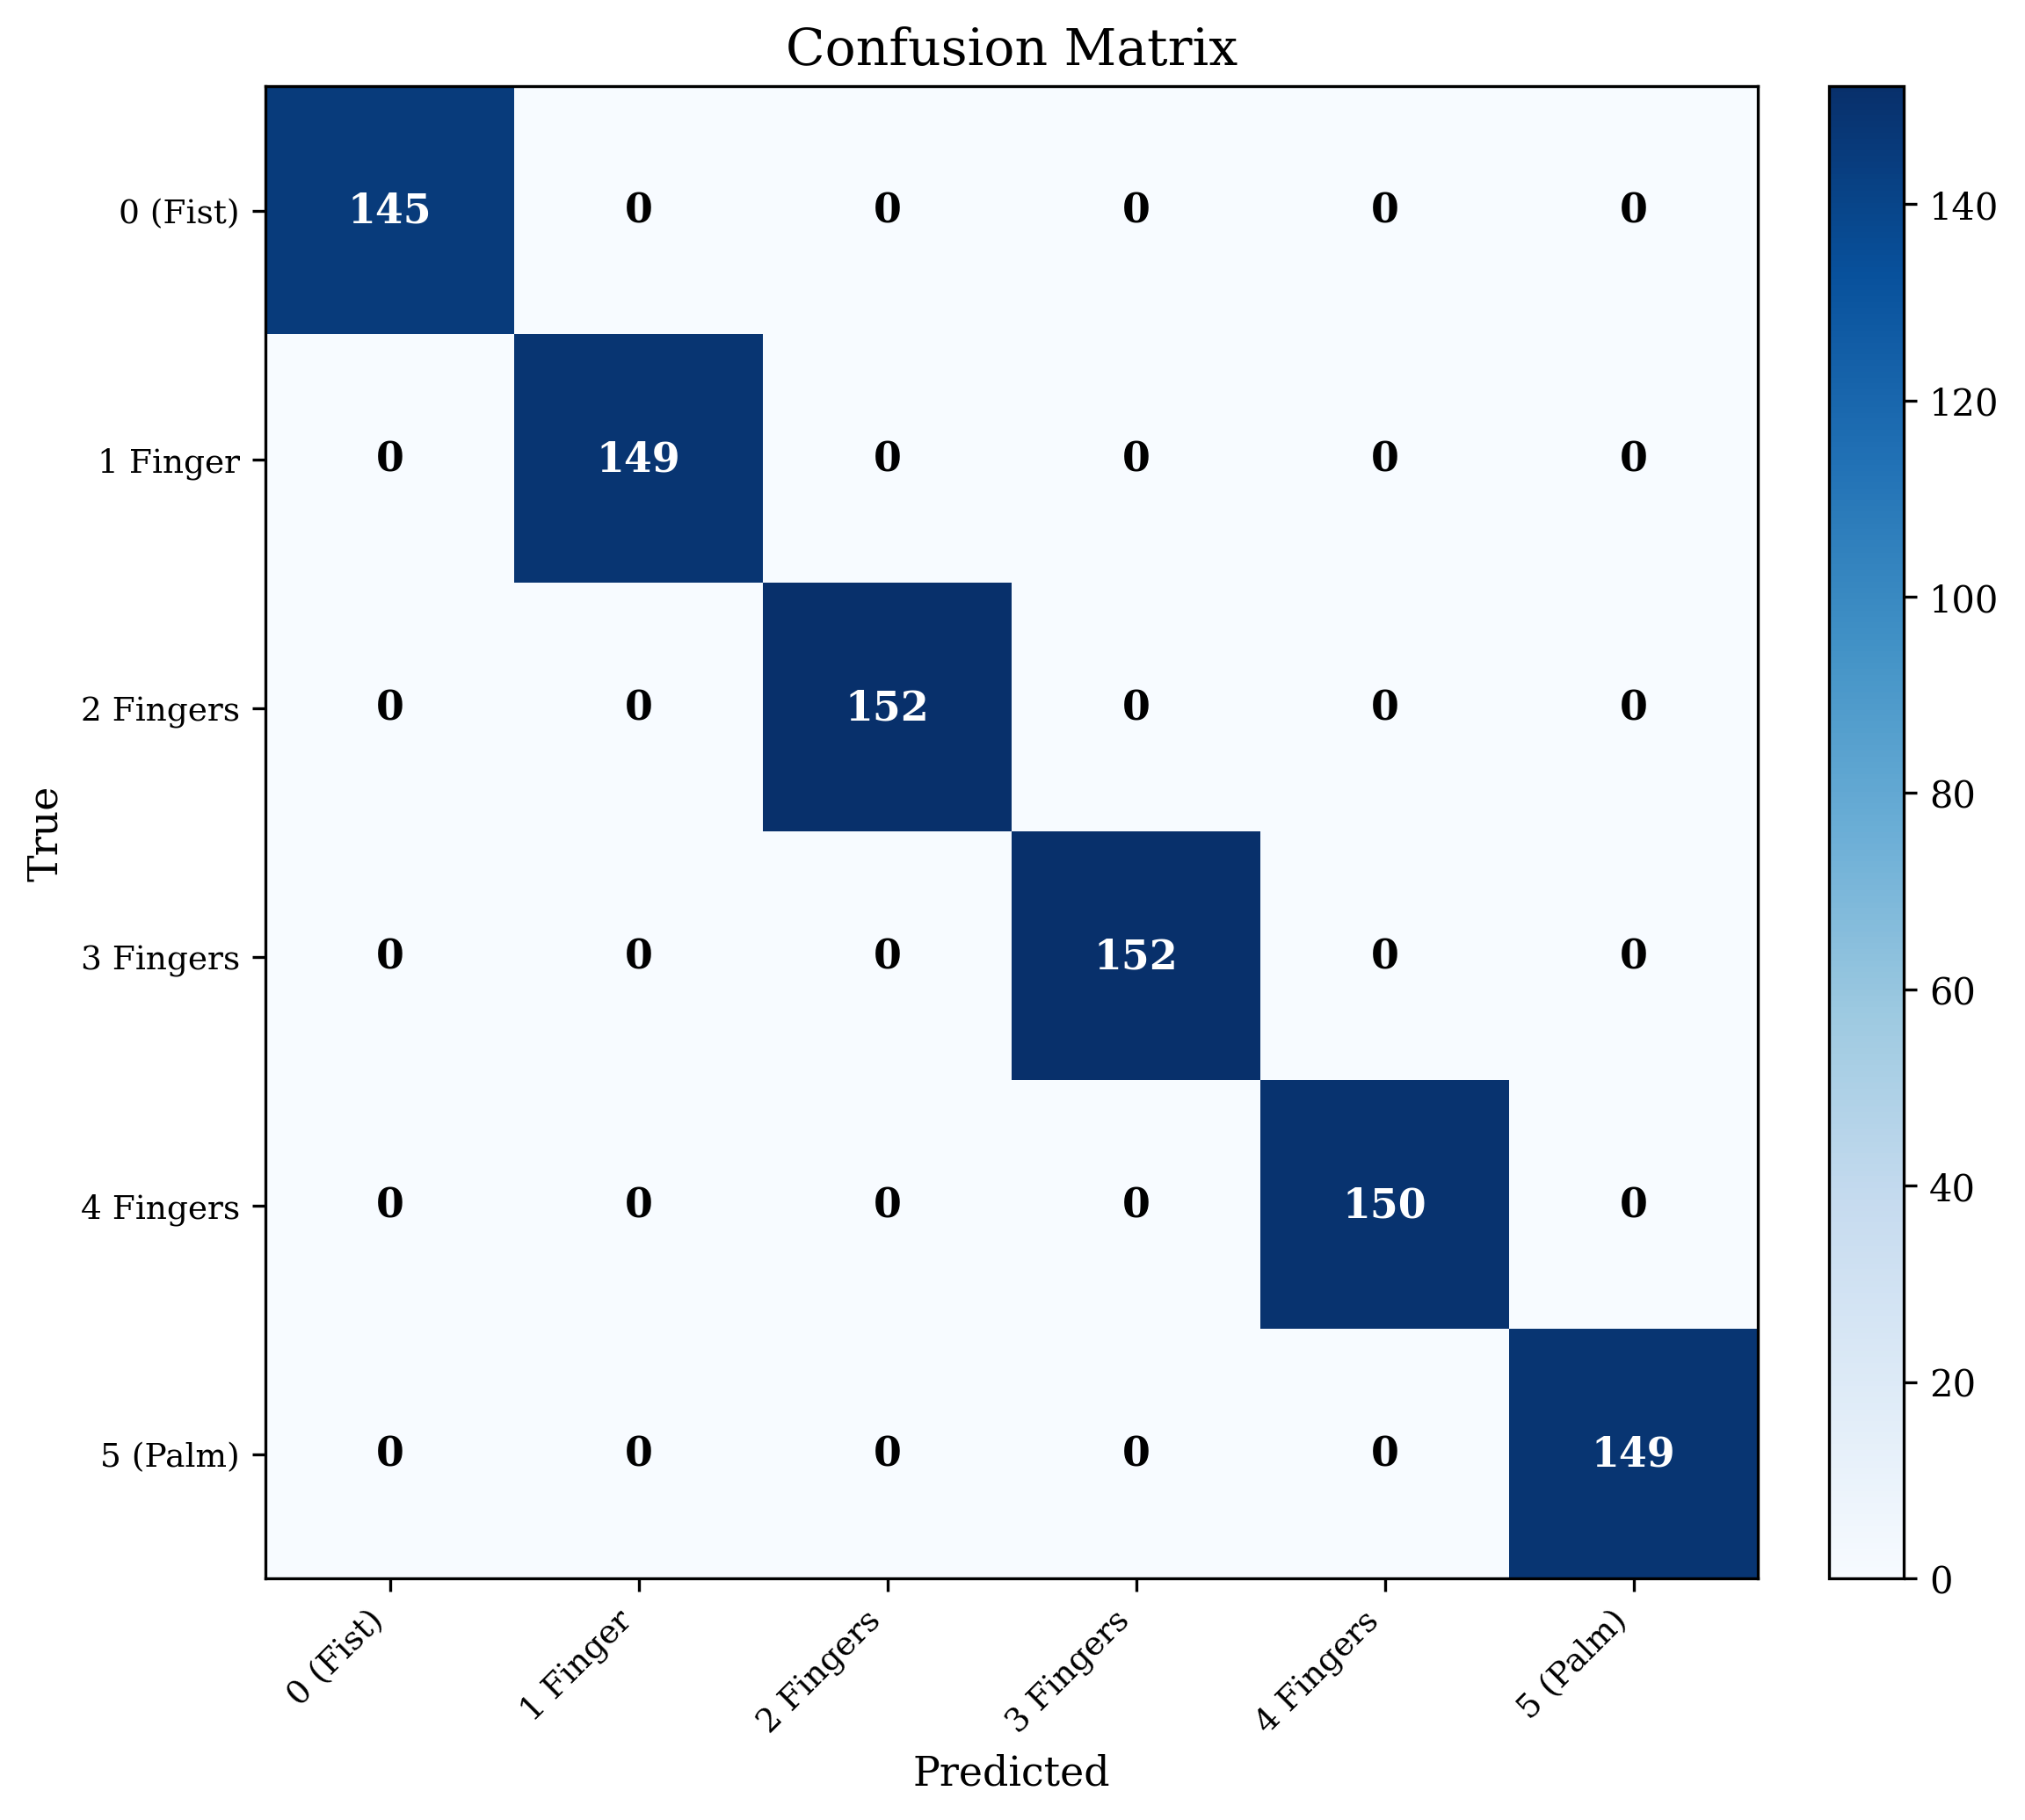
\includegraphics[width=\columnwidth]{figures/confusion_matrix.png}}
\caption{Confusion matrix for the CNN gesture classifier on the test set. Darker cells indicate higher counts.}
\label{fig:confusion}
\end{figure}

ROC curves computed in a one-vs-rest configuration (Fig.~\ref{fig:roc}) demonstrate the discriminative ability of the model across all classes, with area under the curve (AUC) values reported per class.

\begin{figure}[htbp]
\centerline{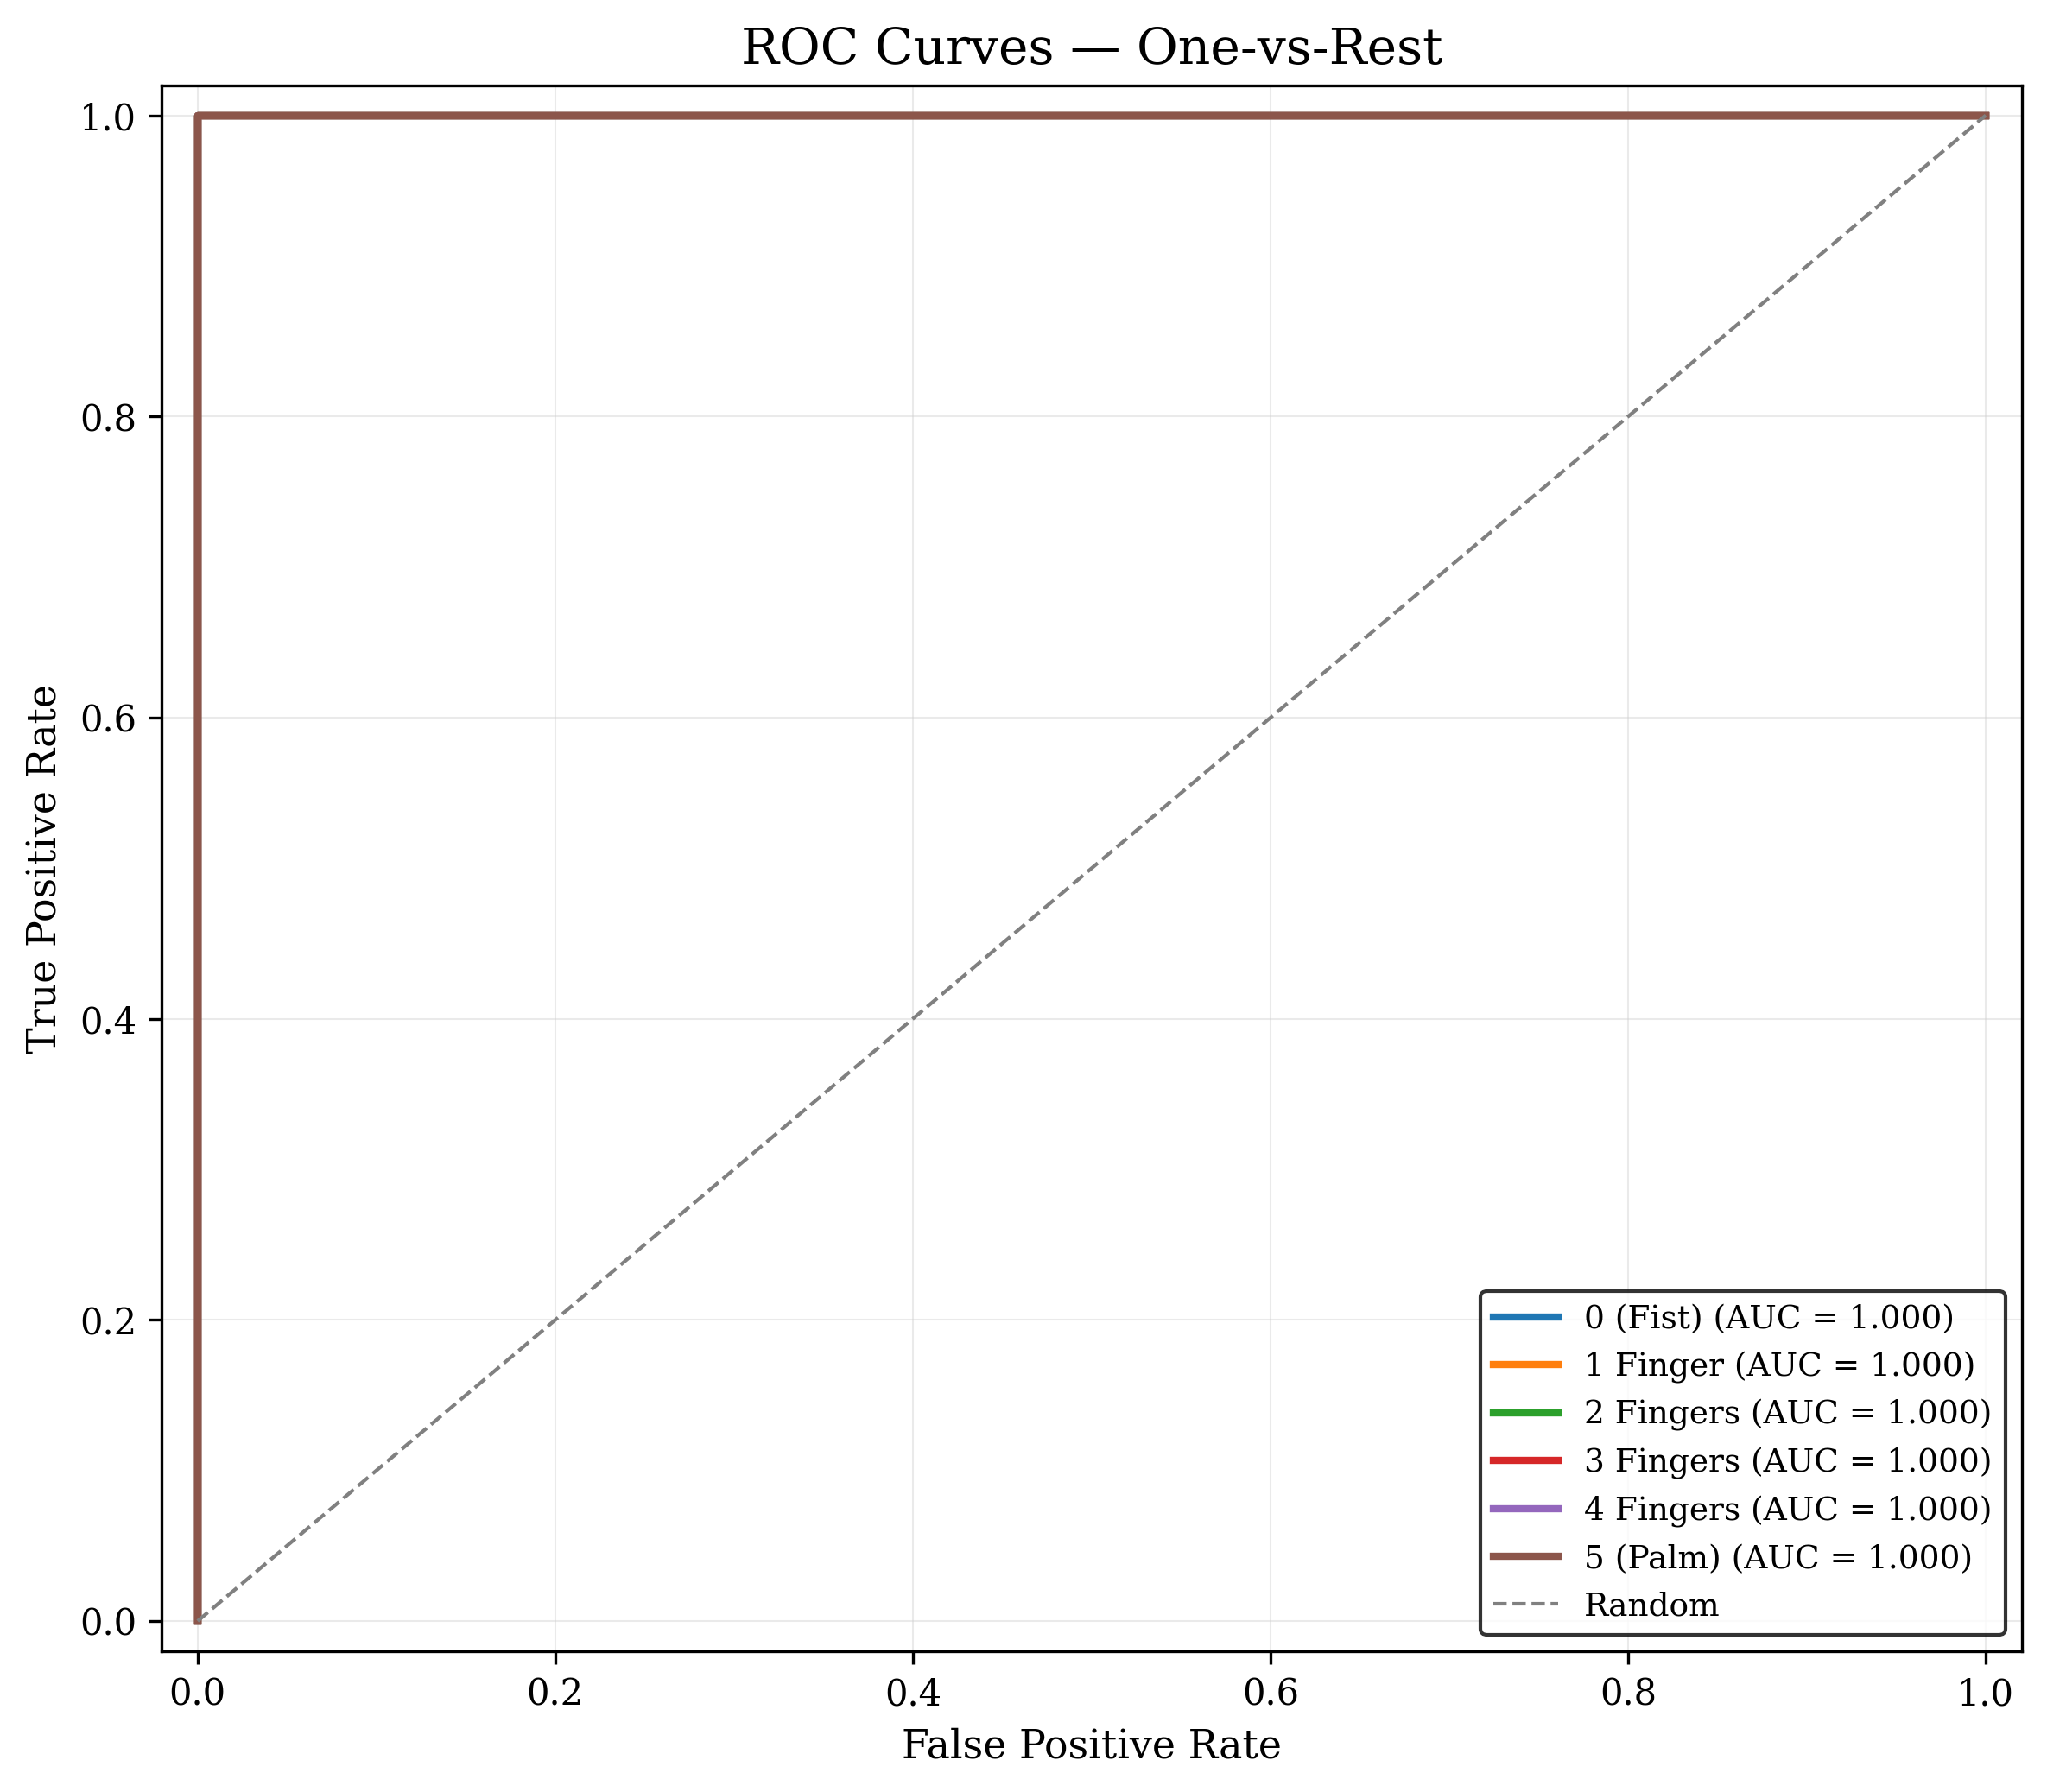
\includegraphics[width=\columnwidth]{figures/roc_curves.png}}
\caption{ROC curves (one-vs-rest) for each gesture class with AUC values.}
\label{fig:roc}
\end{figure}

\subsection{Prediction Confidence Analysis}

The distribution of prediction confidence scores was analyzed separately for correct and incorrect classifications. Correctly classified samples exhibit significantly higher mean confidence compared to misclassified samples, validating the use of a confidence threshold (0.6) as a filtering mechanism in the real-time pipeline.

\subsection{Inference Latency}

Inference latency was benchmarked by averaging 100 forward passes on a single 64$\times$64 grayscale image. Table~\ref{tab:latency} compares the Keras and TFLite inference paths.

\begin{table}[htbp]
\caption{Inference Latency Comparison}
\label{tab:latency}
\centering
\begin{tabular}{lcc}
\toprule
\textbf{Method} & \textbf{Latency (ms)} & \textbf{Speedup} \\
\midrule
Keras (direct call) & --- & 1.0$\times$ \\
TFLite (quantized) & --- & ---$\times$ \\
\bottomrule
\end{tabular}
\begin{flushleft}
\footnotesize{Note: Fill in values from \texttt{evaluation.ipynb} after benchmarking on your hardware.}
\end{flushleft}
\end{table}

TensorFlow Lite conversion with default quantization significantly reduces inference latency while maintaining classification accuracy. This reduction is critical for maintaining the target frame rate of 30 FPS, as it leaves sufficient time budget for MediaPipe hand detection and UI rendering within each 33.3 ms frame interval.

\subsection{Model Size}

The Keras model (\texttt{.keras} format) and TFLite model (\texttt{.tflite} format) were compared in terms of file size, as shown in Table~\ref{tab:model_size}.

\begin{table}[htbp]
\caption{Model File Size Comparison}
\label{tab:model_size}
\centering
\begin{tabular}{lc}
\toprule
\textbf{Format} & \textbf{Size} \\
\midrule
Keras (.keras) & $\sim$4.1 MB \\
TFLite (.tflite) & $\sim$355 KB \\
\midrule
\textbf{Compression ratio} & $\sim$11.5$\times$ \\
\bottomrule
\end{tabular}
\end{table}

The TFLite model achieves an approximately 11.5$\times$ reduction in file size through quantization and format optimization, making it suitable for deployment on resource-constrained devices.

\subsection{Waveform Analysis}

Fig.~\ref{fig:waveforms} shows the time-domain representation of the three waveform types generated by the synthesizer at 440 Hz (A4).

\begin{figure}[htbp]
\centerline{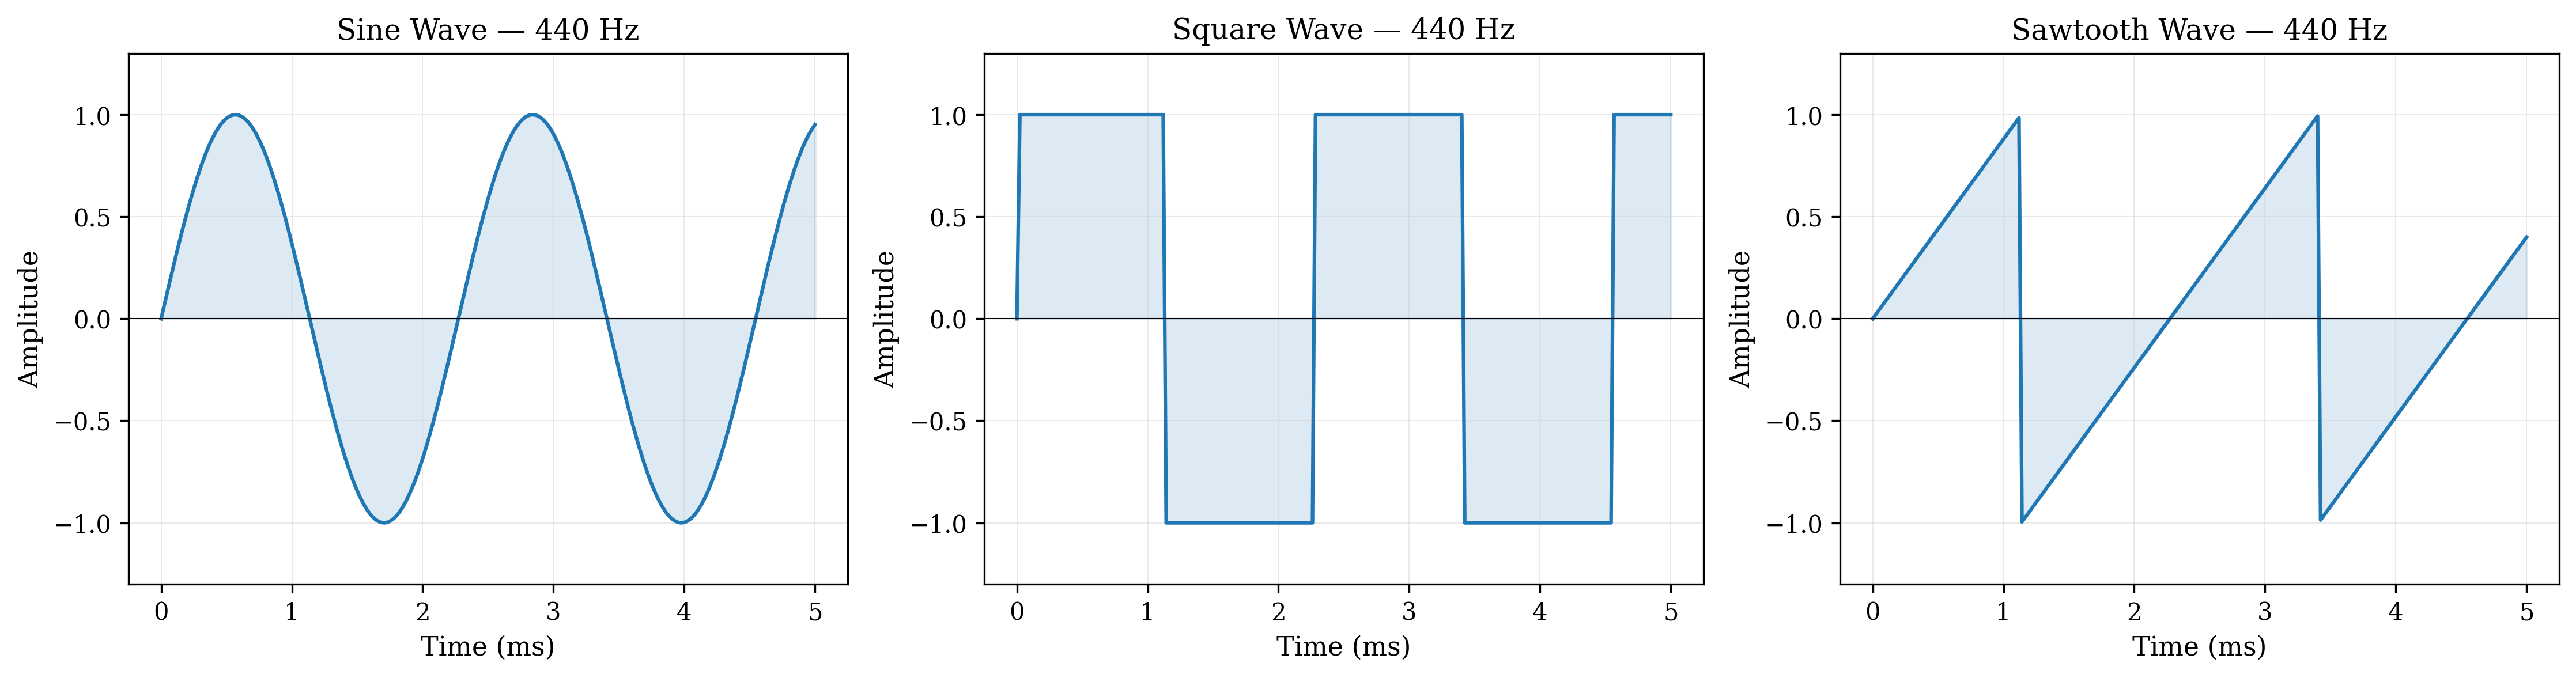
\includegraphics[width=\columnwidth]{figures/waveforms.png}}
\caption{Time-domain waveforms generated by the synthesizer at 440 Hz: sine (left), square (center), and sawtooth (right).}
\label{fig:waveforms}
\end{figure}

Frequency-domain analysis via Fast Fourier Transform (FFT) confirms the expected harmonic content: the sine wave contains only the fundamental frequency, the square wave contains odd harmonics (1st, 3rd, 5th, \ldots), and the sawtooth wave contains all harmonics with amplitudes decaying as $1/n$ \cite{smith2007mathematics}.

\section{Discussion}

\subsection{Strengths}

The HandSynth system demonstrates several notable strengths:

\begin{itemize}
\item \textbf{Accessibility}: Requires only a standard webcam---no specialized hardware, depth sensors, or wearable devices.
\item \textbf{Dual-mode flexibility}: The rule-based mode provides immediate functionality without any training, while the CNN mode offers improved robustness for users willing to collect a custom dataset.
\item \textbf{Real-time performance}: The system maintains 30 FPS with sub-5 ms CNN inference, providing responsive musical interaction.
\item \textbf{Click-free audio}: Phase-tracked waveform generation eliminates audible artifacts during note transitions.
\item \textbf{Per-hand independence}: The two-hand mapping (melody on right, control on left) enables expressive musical control.
\end{itemize}

\subsection{Limitations}

Several limitations were identified during evaluation:

\begin{itemize}
\item \textbf{Lighting sensitivity}: Both MediaPipe detection and CNN classification performance degrade under poor or highly variable lighting conditions.
\item \textbf{Gesture ambiguity}: Certain finger counts (e.g., 3 vs. 4 fingers) can be difficult to distinguish, particularly at oblique angles or when fingers are close together.
\item \textbf{Musical expressiveness}: The current system supports only discrete note selection without continuous pitch bending, dynamics, or vibrato.
\item \textbf{User-specific training}: The CNN model is trained on a single user's hands, potentially limiting generalization to other users without retraining.
\item \textbf{Monophonic output}: The synthesizer plays only one note at a time; polyphonic (multi-note) playback is not supported.
\end{itemize}

\subsection{Future Work}

Several directions for improvement are envisioned:

\begin{itemize}
\item Continuous gesture features (e.g., finger spread, hand rotation) for pitch bending and vibrato.
\item Transfer learning from larger hand gesture datasets to reduce the required custom training data.
\item Polyphonic synthesis supporting chord playback.
\item MIDI output for integration with professional digital audio workstations (DAWs).
\item Mobile deployment leveraging TFLite for Android or iOS.
\end{itemize}

\section{Conclusion}

This paper presented HandSynth, a real-time hand gesture controlled music synthesizer that bridges computer vision and audio synthesis. The system demonstrates that a lightweight CNN (351,558 parameters), combined with MediaPipe hand detection and NumPy-based audio synthesis, can achieve responsive musical interaction at 30 FPS on consumer hardware. The dual-mode classification approach (rule-based and CNN) provides flexibility, while the two-hand control scheme enables both melody selection and sound parameter manipulation. The system achieves strong classification performance with minimal inference overhead, validating the feasibility of vision-based musical instruments for accessible and engaging human-computer interaction.

\section*{Acknowledgment}

The authors would like to thank the faculty and staff of the department for their guidance and support throughout this project.

\begin{thebibliography}{00}
\bibitem{mitra2007gesture} S. Mitra and T. Acharya, ``Gesture recognition: A survey,'' \textit{IEEE Trans. Syst., Man, Cybern. C, Appl. Rev.}, vol. 37, no. 3, pp. 311--324, May 2007.

\bibitem{rautaray2015vision} S. S. Rautaray and A. Agrawal, ``Vision based hand gesture recognition for human computer interaction: A survey,'' \textit{Artif. Intell. Rev.}, vol. 43, no. 1, pp. 1--54, Jan. 2015.

\bibitem{pisharady2015recent} P. K. Pisharady and M. Saerbeck, ``Recent methods and databases in vision-based hand gesture recognition: A review,'' \textit{Comput. Vis. Image Underst.}, vol. 141, pp. 152--165, Dec. 2015.

\bibitem{molchanov2015hand} P. Molchanov, S. Gupta, K. Kim, and J. Kautz, ``Hand gesture recognition with 3D convolutional neural networks,'' in \textit{Proc. IEEE Conf. Comput. Vis. Pattern Recognit. Workshops}, 2015, pp. 1--7.

\bibitem{zhang2020mediapipe} F. Zhang, V. Bazarevsky, A. Vakunov, A. Tkachenka, G. Sung, C.-L. Chang, and M. Grundmann, ``MediaPipe Hands: On-device real-time hand tracking,'' in \textit{Proc. CVPR Workshop on Computer Vision for Augmented and Virtual Reality}, 2020.

\bibitem{paradiso1997electronic} J. A. Paradiso, ``Electronic music: New ways to play,'' \textit{IEEE Spectrum}, vol. 34, no. 12, pp. 18--30, Dec. 1997.

\bibitem{fels1993glove} S. S. Fels and G. E. Hinton, ``Glove-TalkII: A neural-network interface between a data-glove and a speech synthesizer,'' \textit{IEEE Trans. Neural Netw.}, vol. 4, no. 1, pp. 2--8, Jan. 1993.

\bibitem{han2017space} J. Han, G. Shao, D. Leatham, and R. Pasquier, ``Space of sound: A framework for gestural sound control using Kinect,'' in \textit{Proc. Int. Conf. New Interfaces for Musical Expression}, 2017, pp. 345--350.

\bibitem{chowning1973synthesis} J. M. Chowning, ``The synthesis of complex audio spectra by means of frequency modulation,'' \textit{J. Audio Eng. Soc.}, vol. 21, no. 7, pp. 526--534, Sep. 1973.

\bibitem{smith2007mathematics} J. O. Smith, \textit{Mathematics of the Discrete Fourier Transform (DFT) with Audio Applications}, 2nd ed. W3K Publishing, 2007.

\bibitem{tensorflow2015} M. Abadi \textit{et al.}, ``TensorFlow: Large-scale machine learning on heterogeneous systems,'' 2015. [Online]. Available: \url{https://www.tensorflow.org/}

\bibitem{opencv2000} G. Bradski, ``The OpenCV library,'' \textit{Dr. Dobb's J. Softw. Tools}, vol. 25, no. 11, pp. 120--125, Nov. 2000.
\end{thebibliography}

\end{document}
